\documentclass{beamer}
\usepackage{ragged2e}
\usepackage{caption}
\usepackage{color}
\usepackage{tikz}
\usepackage{pstricks}
\usepackage{pst-all}
\usepackage{mathrsfs}
\usepackage{colortbl}
\usepackage{lipsum}
\graphicspath{ {imágenes/} }
\mode<presentation> {
\usetheme{Singapore}

}

\usepackage{graphicx} % Allows including images
\usepackage{subcaption}
\usepackage{booktabs} % Allows the use of \toprule, \midrule and \bottomrule in tables
\usepackage[utf8]{inputenc}
\usepackage[spanish]{babel}
\usepackage{amsmath,amsfonts,amsthm,amssymb}
\DeclareMathOperator{\prox}{prox}

\title[Maestría en Optimización Matemática]{Seminarios} 

\author{\large{
 \underline{Daniela Riera} % Subrayado del expositor
}}
\institute{\large{
Centro de Modelización Matemática (MODEMAT)}
\medskip}
\date{\small{mayo 2026}}

% Fondo para la portada con logos
\addtobeamertemplate{title page}{
    \begin{tikzpicture}[remember picture, overlay]
        % Logo en la esquina inferior izquierda
        \node[anchor=south west, xshift=0.5cm, yshift=0.5cm] 
        at (current page.south west) {
            
\includegraphics[width=2.5cm]{imag_maq/logo1.png}
        };
        % Logo en la esquina inferior derecha
        \node[anchor=south east, xshift=-0.5cm, yshift=1cm] 
        at (current page.south east) {
            
\includegraphics[width=3cm]{imag_maq/logo2.png}
        };
    \end{tikzpicture}
}{}
\justifying
\begin{document}

\begin{frame}
\titlepage % Print the title page as the first slide
\end{frame}
%--------------------------------------------------------------------
\begin{frame}
\frametitle{Índice}
\tableofcontents
\end{frame}
%--------------------------------------------------------------------
\justify
\section{Introducción}
\begin{frame}
\frametitle{Motivación y Formulación del Problema}
Consideremos el problema de optimización {\bf no convexo}: 
\begin{equation*}
        (P)\qquad \displaystyle \min_{u} \frac{1}{2}\|u-y\|^2+\beta \sum_{i=1}^m\|(\mathbb{K}u)_i\|^q,
   \end{equation*}
donde $u\in \mathbb{R}^n$, $q\in(0,1)$, $\beta>0$, $y$ es la imagen contaminada con ruido, $\mathbb{K}:\mathbb{R}^n\to \mathbb{R}^{2m}$ es el gradiente discreto (con respecto a las direcciones $x$ e $y$), es decir, 
$$
(\mathbb{K}u)=(\mathbb{K}_xu, \mathbb{K}_yu), 
$$
donde $\mathbb{K}_x:\mathbb{R}^n\to\mathbb{R}^m$ y $\mathbb{K}_y:\mathbb{R}^n\to \mathbb{R}^m$ corresponden a las derivadas parciales en la dirección horizontal y vertical, respectivamente. 


\end{frame}
%--------------------------------------------------------------------
\justify
\begin{frame}
\frametitle{Motivación y Formulación del Problema}
Para cada $i=1,\ldots,m$
\begin{equation*}
    \|(\mathbb{K}u)_i\|=\left\|(\mathbb{K}_x^iu,\mathbb{K}_y^iu)\right\|=\left\|\left(\begin{array}{c}
        \mathbb{K}_x^i\\
        \mathbb{K}_y^i
    \end{array}\right)u\right\|=\|\mathbb{K}_iu\|,
\end{equation*}
donde $\mathbb{K}_x^i$ y $\mathbb{K}_y^i$ corresponden a la i-ésima fila de $K_x$ y $K_y$, respectivamente.\vspace{0.5cm}
\end{frame}
%--------------------------------------------------------------------
\begin{frame}
\frametitle{Motivación y Formulación del Problema}
\textbf{La incorporación de la penalización $TVq$}
$$
\sum_{i=1}^m\|(\mathbb{K}u)_i\|^q
$$
\textbf{ayuda preservar de mejor manera los bordes presentes en la imagen y reducir el efecto de escalonamiento (staircasing effect)} que es común cuando se utiliza la variación total ($TV$).
\end{frame}
%--------------------------------------------------------------------
\justify
\section{Tratamiento del Problema}
\begin{frame}
\frametitle{Tratamiento del Problema}
El problema $(P)$ es \textbf{no convexo} y \textbf{no diferenciable}, por lo que introducimos una regularización de tipo Huber. Para $\gamma\gg1$ definimos
\begin{equation*}
    h_{q,\gamma}(t) = \left\{\begin{array}{ll}
        q\gamma^{\frac{1-q}{q}}|t|^{\frac{1}{q}} & |t|\leq \frac{1}{\gamma}, \\ \\
        |t|+\frac{q-1}{\gamma}                   & |t|>\frac{1}{\gamma}.
    \end{array}\right.
\end{equation*}

\rule{\linewidth}{0.4pt} % Línea horizontal de ancho total y grosor 0.4pt
{\tiny
La regularización $h_{p,\gamma}$ (donde $p=1/q$) está definida en Merino, P. (2019). A difference-of-convex functions approach for sparse PDE optimal control problems with nonconvex costs. \textit{Computational Optimization and Applications}, 74(1), 225-258.
}
\end{frame}
%--------------------------------------------------------------------
\justify
\begin{frame}
\frametitle{Tratamiento del Problema}
Luego, 
    \begin{equation*}
        (h_{q,\gamma}(t))^q = \left\{\begin{array}{ll}
           \delta_{\gamma}|t|, & |t|\leq \frac{1}{\gamma},\\\\
           \left(|t|+(q-1)/\gamma\right)^q, & |t|>\frac{1}{\gamma},
            \end{array}\right.
    \end{equation*}
donde $\delta_{\gamma}:=q^q\gamma^{1-q}$.
\end{frame}

%-------------------------------------------------------------------------------
\justify
\begin{frame}
\frametitle{Tratamiento del Problema}
De este modo, el problema (P) es aproximado por el problema parametrizado por $\gamma$:
\begin{equation*}
    (P_{\gamma})\qquad \min_{u} \frac{1}{2}\|u-y\|^2+\beta\sum_{i=1}^m(h_{q,\gamma}(\|(\mathbb{K}u)_i\|))^q.
\label{reg}
\end{equation*}
\end{frame}
%-------------------------------------------------------------------
\justify
\begin{frame}
\frametitle{Condiciones de Optimalidad}

Reformulamos ($P_{\gamma}$) como la minimización de la diferencia de dos 
funciones convexas: $G$ y $H$. 
\begin{align*}
&\begin{array}{ll}
     G:& \mathbb{R}^n\to \mathbb{R} \\
     &u \mapsto \displaystyle \frac{1}{2}\|u-y\|^2+\delta_{\gamma}\beta\sum_{i=1}^m\|(\mathbb{K}u)_i\|, 
\end{array}\\
&\begin{array}{ll}
    H:& \mathbb{R}^n\to \mathbb{R} \\
     &u \mapsto \beta\left(\displaystyle\sum_{i=1}^m[\delta_{\gamma}\|(\mathbb{K}u)_i\|-(h_{q,\gamma}(\|(\mathbb{K}u)_i\|))^q]\right).
\end{array}
\end{align*}
Es decir, $(P_{\gamma})$ es equivalente a
$$
\min_{u} G(u)-H(u).
$$
\end{frame}
%-------------------------------------------------------------------
\justify
\begin{frame}{Condiciones de Optimalidad}
La función $j:\mathbb{R}_+\cup \{0\}\to \mathbb{R}_+\cup \{0\}$, definida por
\begin{equation*}
    j(t)=\left\{\begin{array}{ll}
        \beta \delta_{\gamma}t- \beta\left(t+\frac{q-1}{\gamma}\right)^q & t > \frac{1}{\gamma},\\ \\
       0 & t\leq\frac{1}{\gamma}
    \end{array}\right.
\end{equation*}
es no negativa, convexa, continuamente diferenciable y su derivada está dada por
\begin{equation*}
    j'(t)=\left\{\begin{array}{ll}
       \beta\delta_{\gamma}-\beta q\left(t+\frac{q-1}{\gamma}\right)^{q-1}  &  t >\frac{1}{\gamma}, \\\\
         0&t\leq \frac{1}{\gamma}.
    \end{array}\right.
    \label{jprima}
\end{equation*} 
\end{frame}
%-------------------------------------------------------------------
\justify
\begin{frame}{Condiciones de Optimalidad}
Usando la función $j$, podemos escribir  $H$ como sigue:
\begin{align*}
    H:\mathbb{R}^n&\to \mathbb{R}\\
    u &\mapsto \sum_{i=1}^mj(\|(\mathbb{K}u)_i\|).
\end{align*}
\end{frame}
%-------------------------------------------------------------------
\justify
\begin{frame}{Condiciones de Optimalidad}
Las funciones $G$ y $H$ son convexas.
\begin{align*}
    \begin{array}{ll}
         G:& \mathbb{R}^n\to \mathbb{R} \\
         &u \mapsto \displaystyle\frac{1}{2}\|u-y\|^2+\delta_{\gamma}\beta\sum_{i=1}^m\|(\mathbb{K}u)_i\|, 
    \end{array}\;
    \begin{array}{ll}
        H:& \mathbb{R}^n\to \mathbb{R} \\
         &u \mapsto \displaystyle\sum_{i=1}^mj(\|(\mathbb{K}u)_i\|).
    \end{array}
    \end{align*}
En efecto, puesto que $\displaystyle \frac{1}{2}\|\cdot\|^2$ es estrictamente convexa, $\delta_{\gamma}\beta>0$, $\|\cdot\|$ es convexa y la suma
preserva la convexidad, por tanto $G$ es estrictamente convexa. Dado que $j$ es convexa, $H$ es convexa. 
\end{frame}
%-------------------------------------------------------------------
\justify
\begin{frame}{Condiciones de Optimalidad}
Usando la programación DC (difference of convex functions), tenemos que si $u^*$ es un mínimo local para $(P_\gamma)$, entonces $u^*$ satisface la condición de criticalidad: $$\partial H(u^*)\subset \partial G(u^*),$$
donde $\partial H$ y $\partial G$ corresponden a los subdiferenciales de $H$ y $G$, respectivamente.  
\end{frame}
%-------------------------------------------------------------------
\justify
\begin{frame}{Condiciones de Optimalidad}
La función $H$ es Gâteaux diferenciable y su derivada es 
    \begin{align*}
   \nabla H(u)&=\mathbb{K}^Tw,
  \end{align*}
  donde $w=D_a\mathbb{K}u\in\mathbb{R}^{2m}$, $D_a=diag(a_1,a_2,\ldots,a_m,a_1,a_2,\ldots,a_m)$ es una matriz diagonal en $\mathbb{R}^{2m\times 2m},$ 
  \begin{equation*}
  a_i=\hat{j}(\|(\mathbb{K}u)_i\|)=\left\{\begin{array}{ll}
    \displaystyle \frac{j'(\|(\mathbb{K}u)_i\|)}{\|(\mathbb{K}u)_i\|}&\|(\mathbb{K}u)_i\|>\frac{1}{\gamma},\\\\
    0&\|(\mathbb{K}u)_i\|\leq \frac{1}{\gamma}.
  \end{array}\right.
  \end{equation*} y $$\mathbb{K}u=[\mathbb{K}_x^1u,\ldots \mathbb{K}_x^mu,\mathbb{K}_y^1u,\ldots,\mathbb{K}_y^mu]^T\in \mathbb{R}^{2m}.$$
\end{frame}
%------------------------------------------------------------------------------
\begin{frame}
\frametitle{Condiciones de Optimalidad}
Si $u^*$ es una solución de $(P_\gamma)$, entonces $u^*$ satisface el siguiente sistema de optimalidad: 
\begin{align*}
    \mathbb{K}^Tw-u^*+y-\delta_{\gamma}\sum_{i=1}^m\mathbb{K}_i^Tz_i=0,\\
    z_i \in \beta\partial\|\cdot\|((\mathbb{K}u^*)_i), \quad \forall i=1,\ldots,m.
\end{align*}
\end{frame}
%-------------------------------------------------------------------------------
\begin{frame}
\frametitle{Condiciones de Optimalidad}
\textit{Idea de la demostración.}
\begin{itemize}
    \justifying
    \item Tomamos $u^*$ una solución de $(P_{\gamma})$.
    \item Calculamos $\partial G(u^*)=\left\{u^*-y+\delta_{\gamma}\displaystyle\sum_{i=1}^m \mathbb{K}_i^T z_i\right\},$ donde
 \begin{align*}
z_i\in \beta\partial\|\cdot\|((\mathbb{K}u^*)_i)=\left\{\begin{array}{ll}
\displaystyle\frac{\beta(\mathbb{K}u)_i}{\|(\mathbb{K}u)_i\|}& (\mathbb{K}u)_i\neq 0, \\\\
             \beta clB_*(0,1)& (\mathbb{K}u)_i=0.
        \end{array}\right.
 \end{align*}
\item Tomamos $h\in \partial H(u^*)=\{\nabla H(u^*)\}$, así $h=\mathbb{K}^Tw$. De la condición de criticalidad ($\partial H(u^*)\subset \partial G(u^*)$), $h\in \partial G(u^*)$.
  \end{itemize}
\end{frame}
%--------------------------------------------------------------------
\begin{frame}
    \frametitle{Condiciones de Optimalidad}
\begin{itemize}
    \item Como $h\in \partial G(u^*),$ 
    $$
    h=u^*-y+\delta_{\gamma}\displaystyle\sum_{i=1}^m \mathbb{K}_i^T z_i.
    $$
    \item Finalmente,
  \begin{align*}
     &\mathbb{K}^Tw=u^*-y+\delta_{\gamma}\sum_{i=1}^m \mathbb{K}_i^Tz_i,\\
     \Rightarrow &\mathbb{K}^Tw-u^*+y-\delta_{\gamma}\sum_{i=1}^m \mathbb{K}_i^Tz_i=0.
  \end{align*} 
\end{itemize}
\end{frame}
%--------------------------------------------------------------------
\justify
\section{Algoritmo DC Primal-Dual}
\begin{frame}
\frametitle{Algoritmo DC Primal-Dual}
 Para resolver numéricamente el problema $(P_\gamma)$ proponemos combinar el DCA - Primal-Dual Hybrid Gradient: 
 \vspace{0.5cm}
 {\sffamily
\begin{enumerate}
    \item Choose $\sigma>0$, $\tau>0$, $\theta$, $q$ , $\gamma$
    \item Initialize $u_0$,$\bar u_0$, $y_0$; set $k=0$
    \item \textbf{repeat} Until DC stopping criteria is satisfied
    \item \quad Compute $\mathbb{K}^Tw_k\in \partial H(u_k)$
    \item \quad Compute $u_k\in \partial G^*(\mathbb{K}^Tw_k)=argmin_{u_k}\{G(u_k)-\langle \mathbb{K}^Tw_k,u_k\rangle\}$
    \item \textbf{end}
\end{enumerate}}
\end{frame}
%-------------------------------------------------------------------
\justify
\begin{frame} 
\frametitle{Algoritmo DC Primal-Dual}
Notemos que el paso 5 es equivalente a resolver el siguiente problema:
$$
\min_{u_k} -\langle \mathbb{K}^Tw_k,u_k\rangle+\frac{1}{2}\|u_k-y\|^2+\delta_{\gamma}\beta\displaystyle \sum_{i=1}^m\|(\mathbb{K}u_k)_i\|.
$$
El cual es equivalente a 
$$
\min_{u_k} -\frac{1}{\beta\delta_{\gamma}}\langle\mathbb{K}^Tw_k,u_k\rangle+\frac{1}{2\delta_{\gamma}\beta}\|u_k-y\|^2+\sum_{i=1}^m\|(\mathbb{K}u_k)_i\|.
$$
\end{frame}
%-------------------------------------------------------------------
\justify
\begin{frame} 
\frametitle{Algoritmo DC Primal-Dual}
Tomando 
$$\displaystyle F(u_k):=\frac{1}{2\beta\delta_{\gamma}}\|u_k-y\|^2-\frac{1}{\delta_{\gamma}\beta}\langle \mathbb{K}^Tw_k,u_k\rangle\;\text{y}\;G(\mathbb{K}u):=\|\mathbb{K}u\|_1,$$ donde $\|\mathbb{K}u\|_1=\displaystyle\sum_{i=1}^m\|(\mathbb{K}u)_i\|$, obtenemos el siguiente problema
$$
\min_{u_k} F(u_k)+G(\mathbb{K}u_k).
$$
\end{frame}
%-------------------------------------------------------------------
\justify
\begin{frame} 
\frametitle{Algoritmo DC Primal-Dual}
Para resolverlo, usamos el algoritmo Primal Dual Hybrid Gradient (PDHG) para resolver el paso 5:
\vspace{0.5cm}
\begin{enumerate}
    \item [5.1]\textbf{while} Until stopping criteria is satisfied \textbf{do}
    \item [5.2]\quad $p_{k+1} = \prox_{\sigma G^*}(p^k+\sigma \mathbb{K}\bar{u}_{k})$
    \item [5.3]\quad $u_{k+1} = \prox_{\tau F}(u^k-\tau \mathbb{K}^*p^k)$
    \item [5.4]\quad $\bar{u}_{k+1} = {u}_{k+1} + \theta({u}_{k+1}-{u}_{k})$
    \item [5.5]\textbf{end}
\end{enumerate}
\end{frame}

%-------------------------------------------------------------------
\justify
\begin{frame} 
\frametitle{Experimentación Numérica}
¿Qué sucede si aumentamos el valor de $\beta$? 
\begin{figure}[H]
\centering 
\begin{subfloat}{
    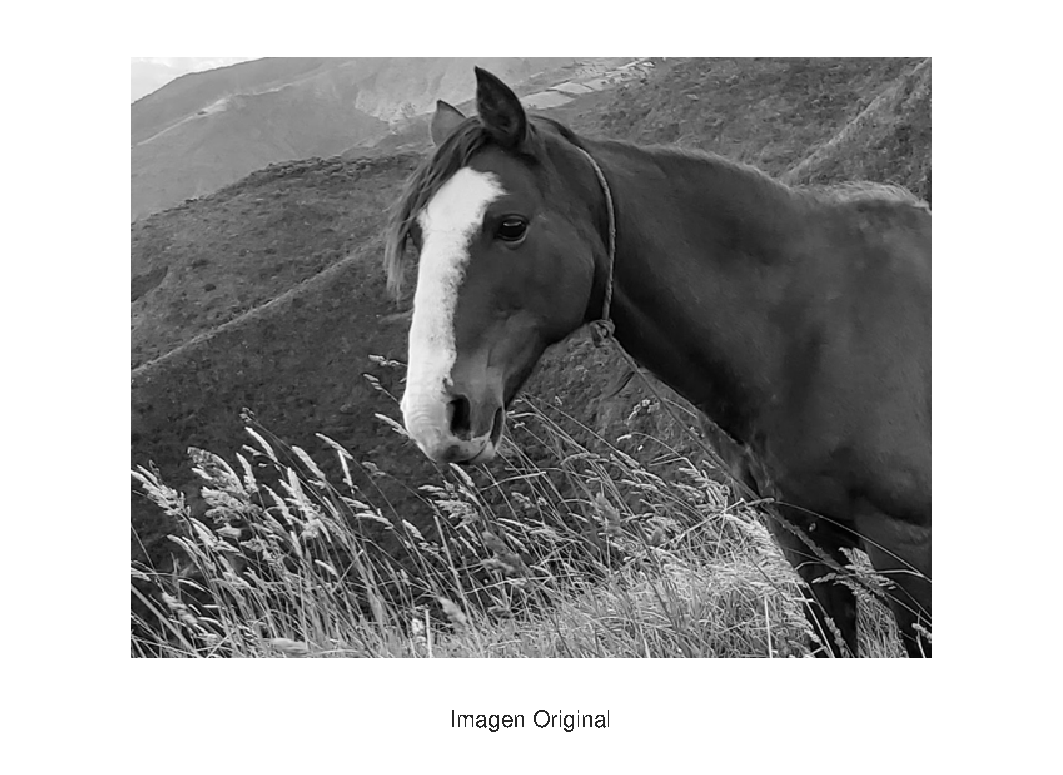
\includegraphics[scale=0.28]{imag_maq/cab_or.eps}
}
\end{subfloat}\vspace{0.01cm}
\begin{subfloat}{
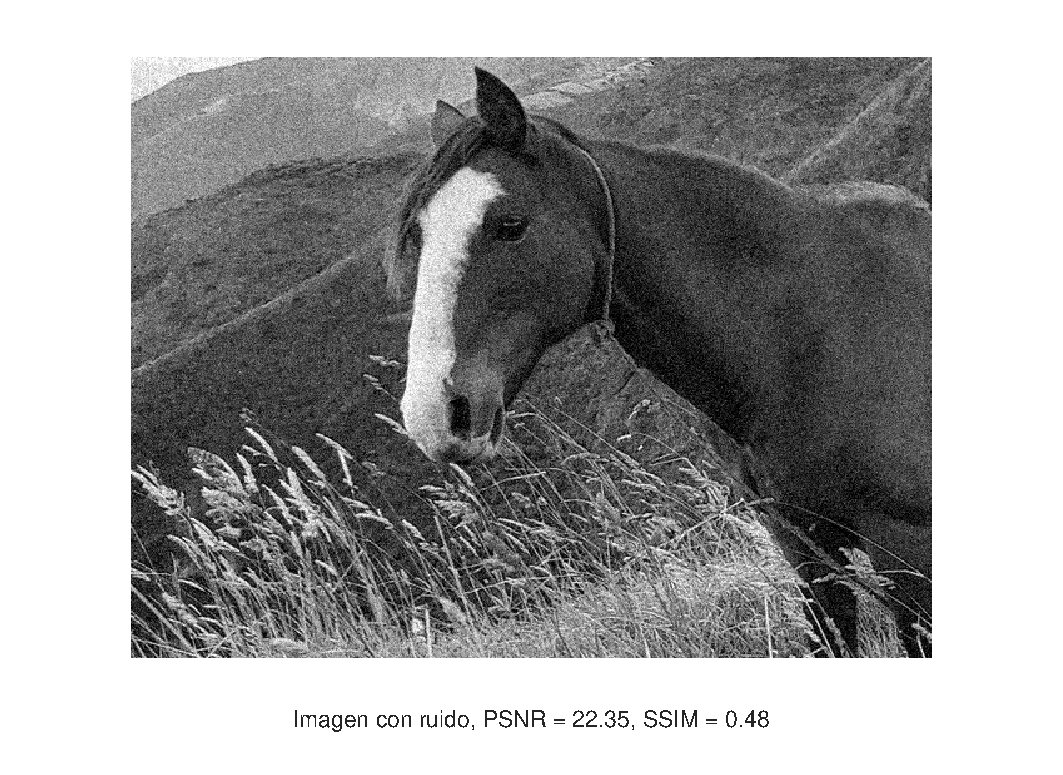
\includegraphics[scale=0.28]{imag_maq/cab_ruido.eps}
}
\end{subfloat}\\
\begin{subfloat}{
    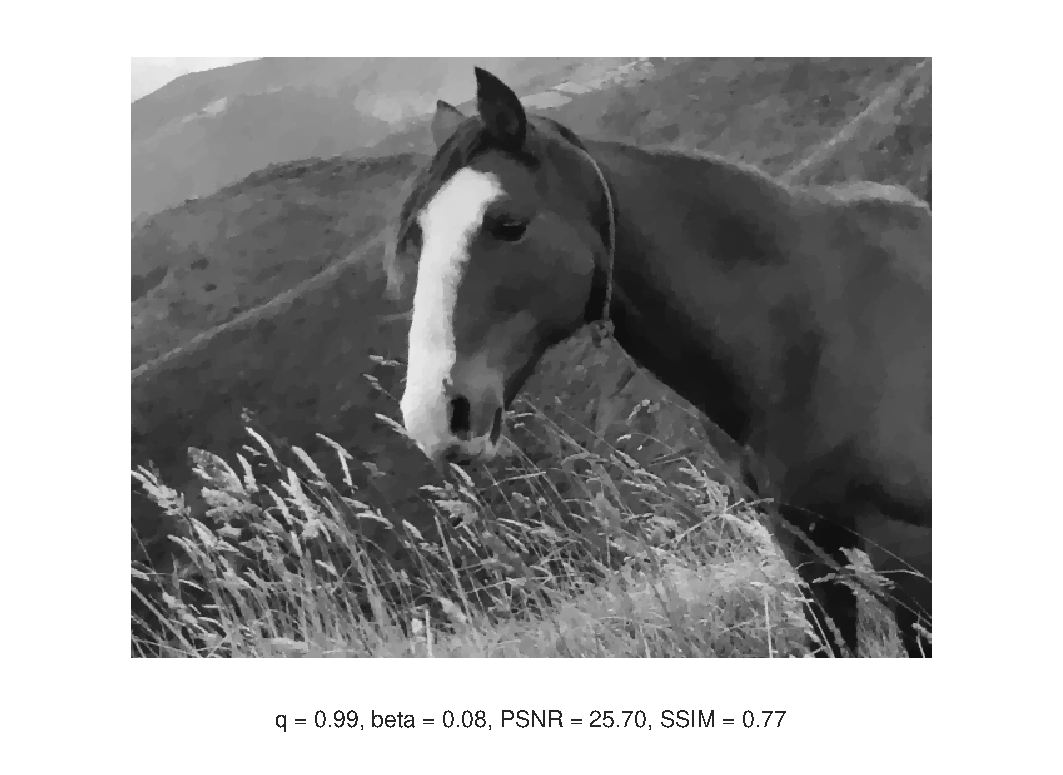
\includegraphics[scale=0.28]{imag_maq/cab_ruido_q09_beta008.eps}
    }
    \end{subfloat}
\begin{subfloat}{
        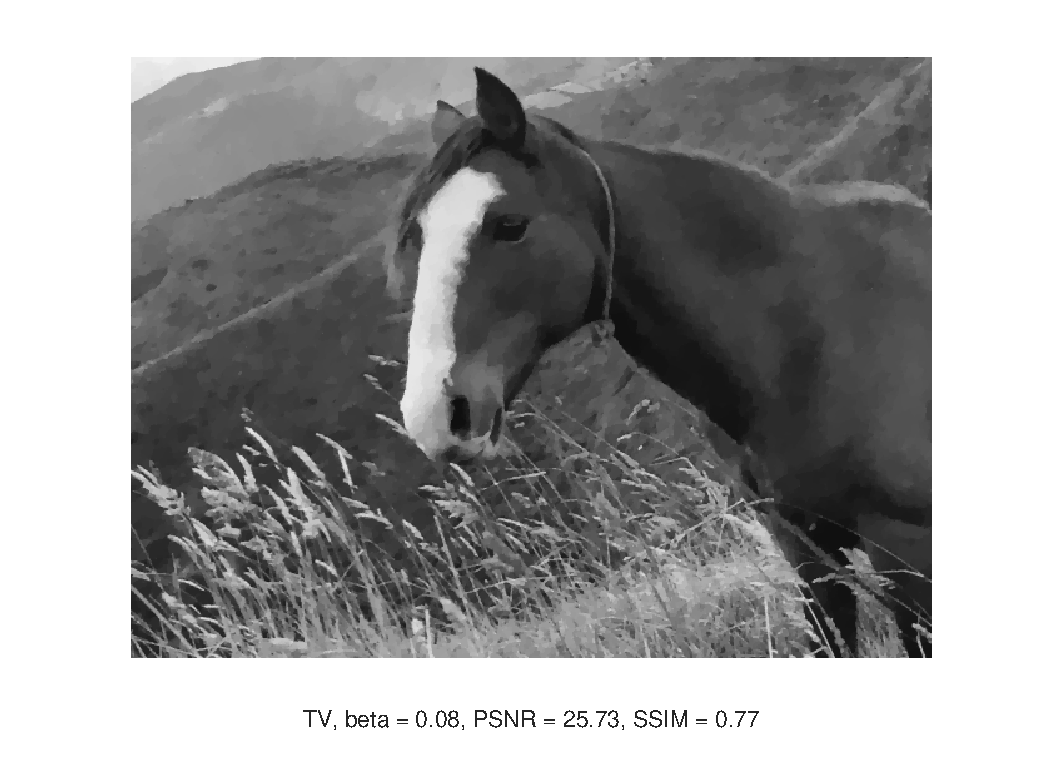
\includegraphics[scale=0.28]{imag_maq/cab_ruido_lambda008.eps}
        }
        \end{subfloat}
\end{figure}

\end{frame}

%--------------------------------------------------------------------
\begin{frame}
\section{Conclusiones}
\frametitle{Conclusiones y Trabajo en Progreso}
\begin{itemize}
    \justifying
        \item La elección de los parámetros $q$ y $\beta$ influye de manera determinante en la calidad de los resultados y en el costo computacional. Es por ello que planteamos un \textbf{problema binivel}, que 
   nos permita encontrar el valor de $\beta$ óptimo. Puesto que, los experimentos numéricos muestran un valor grande de $\beta$, pueden causar un sobre suavizado de la imagen. 
 \begin{equation*}
    (PB_{\gamma}) \left\{\begin{array}{l}
        \displaystyle \min_{(u,\beta)\in \mathbb{R}^n\times \mathbb{R}_+}  J(u) \\
        \text{sujeto a}                                                             \\
        \left\{\begin{array}{l}
                   \displaystyle \min_{u} \frac{1}{2}\|u-y\|^2+\beta \sum_{i=1}^m h_{q,\gamma}(\|(\mathbb{K}u)_i\|)^q.
               \end{array}\right.
    \end{array}\right.
\end{equation*}
   \item Una vez planteado el problema Binivel, se demostrarán condiciones de calificación particulares y se resolverá numéricamente utilizando un algoritmo de punto interior. 
\end{itemize}
\end{frame}
\end{document}